\documentclass[handout]{beamer}
 
\usepackage[utf8]{inputenc}
\usepackage{mathtools}
\usepackage{tikz}
\usetikzlibrary{calc}

\usetheme{CambridgeUS}
\useoutertheme{split}
\setbeamertemplate{title page}[default][colsep=-4bp,rounded=true]
 
%Information to be included in the title page:
\title{Authenticated Encryption}
\author{Rohit Musti}
\institute{CUNY - Hunter College}
\date{\today}
 
\begin{document}
 
\frame{\titlepage}

\begin{frame}
    \frametitle{Authenticated Encryption Motivation}
    \begin{itemize}
      \item \pause Up until now we have considered systems that provide either message secrecy or integrity separately\pause
      \item A system is said to provide authenticated encryption if it provides both message secrecy and integrity! \pause
      \item At the end of this lecture, you will be empowered to analyze and construct authenticated encryption systems!
    \end{itemize}
\end{frame}

\begin{frame}
  \frametitle{Basic Authenticated Encryption System}
  \begin{itemize}
    \item \pause We can use generic composition techniques to combine separate encryption and integrity schemes into an authenticated encryption scheme \pause
    \item Let \(E,D\) be a cipher, \(k_c\) be the cipher key, \(S,V\) be a MAC, and \(k_m\) be the MAC key \pause
    \item An integrated scheme builds directly ontop of cryptographic primitives without first constructing either a cipher of a MAC
  \end{itemize}
\end{frame}


\begin{frame}
    \frametitle{Cipher Text Integrity Game}
    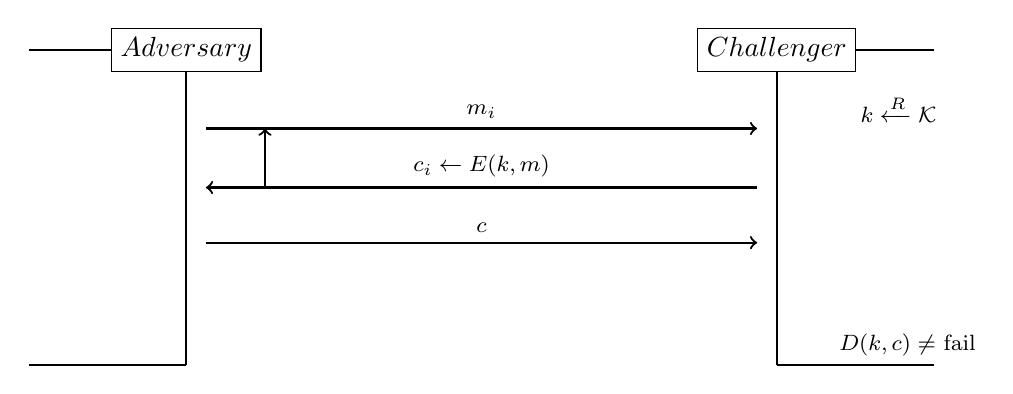
\begin{tikzpicture}
        \node[draw] (Adversary) at (-3, 2) {\(Adversary\)}; 
        \draw[thick] (Adversary) -- ++(0, -4); 
        \draw[thick] (Adversary) -- ++(-2, 0);
        \draw[thick] (-3, -2) -- ++(-2, 0);
        
        \pause

        \node[draw] (Challenger) at (4.5,2) {\(Challenger\)}; 
        \draw[thick] (Challenger) -- ++(0, -4);
        \draw[thick] (Challenger) -- ++(2, 0);
        \draw[thick] (4.5, -2) -- ++(2, 0);

        \pause

        \node[draw=none,fill=none,anchor=east, font=\footnotesize] (choice0) at ($(Challenger) + (2.15,-.75)$) {\(k \xleftarrow{R} \mathcal{K}\)};

        \pause

        \draw[->,thick] ($(Adversary)+(0.25,-1)$) -- ($(Challenger)+(-0.25,-1)$) node [pos=0.5,above,font=\footnotesize] {\(m_i\)};

        \pause

        \draw[->,thick] ($(Challenger)+(-0.25,-1.75)$) -- ($(Adversary)+(0.25,-1.75)$) node [pos=0.5,above,font=\footnotesize] {\(c_i \leftarrow E(k, m)\)};

        \pause

        \draw[->,thick] ($(Adversary)+(1,-1.75)$) -- ($(Adversary)+(1,-1)$);

        \pause

        \draw[->,thick] ($(Adversary)+(0.25,-2.45)$) -- ($(Challenger)+(-0.25,-2.45)$) node [pos=0.5,above,font=\footnotesize] {\(c\)};


        \node[draw=none,fill=none,anchor=east, font=\footnotesize] (choice0) at ($(Challenger) + (2.65,-3.75)$) {\(D(k, c) \neq \) fail};
      \end{tikzpicture} 
\end{frame}

\begin{frame}
  \begin{itemize}
    \frametitle{Why is Cipher Text Integrity important?}
    \item \pause Suppose Alice emails Bob and every message starts with "To:bob@aol.com" and the mail servers knows to forward the plaintext message encrypted with Bob's key to Bob \pause
    \item An attacker can intercept the message and modify the beginning to say "To: attacker@aol.com", the mail server will then forward the plaintext message encrypted with the Attacker's key to the Attacker \pause
    \item If we an AE cipher (aka cipher text integrity secure cipher), then Mel cannot produce a valid modified cipher text
  \end{itemize}
  
\end{frame}

\begin{frame}
    \frametitle{Chosen Ciphertext Attack (CCA) Game}
    \text{} \\
      \[ V(k,m,t) = S(k,m) == t \] \pause
    \bigskip
    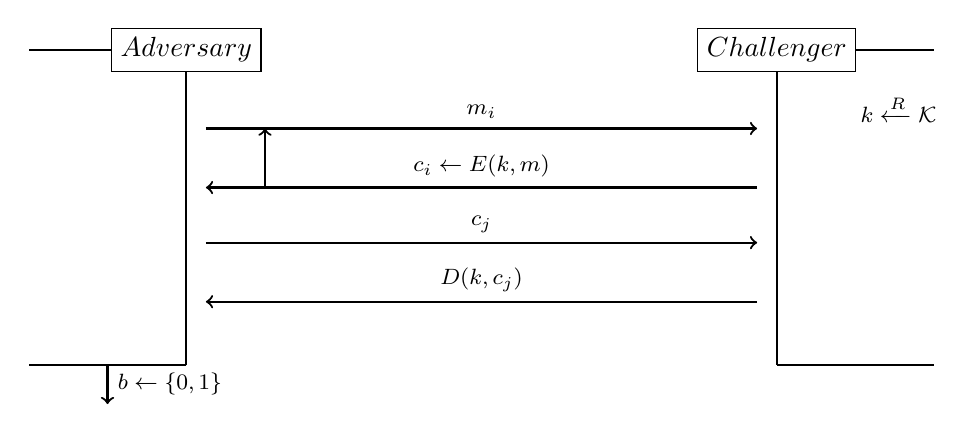
\begin{tikzpicture}
        \node[draw] (Adversary) at (-3, 2) {\(Adversary\)}; 
        \draw[thick] (Adversary) -- ++(0, -4); 
        \draw[thick] (Adversary) -- ++(-2, 0);
        \draw[thick] (-3, -2) -- ++(-2, 0);
        
        \pause

        \node[draw] (Challenger) at (4.5,2) {\(Challenger\)}; 
        \draw[thick] (Challenger) -- ++(0, -4);
        \draw[thick] (Challenger) -- ++(2, 0);
        \draw[thick] (4.5, -2) -- ++(2, 0);

        \pause

        \node[draw=none,fill=none,anchor=east, font=\footnotesize] (choice0) at ($(Challenger) + (2.15,-.75)$) {\(k \xleftarrow{R} \mathcal{K}\)};

        \pause

        \draw[->,thick] ($(Adversary)+(0.25,-1)$) -- ($(Challenger)+(-0.25,-1)$) node [pos=0.5,above,font=\footnotesize] {\(m_i\)};

        \pause

        \draw[->,thick] ($(Challenger)+(-0.25,-1.75)$) -- ($(Adversary)+(0.25,-1.75)$) node [pos=0.5,above,font=\footnotesize] {\(c_i \leftarrow E(k, m)\)};

        \pause

        \draw[->,thick] ($(Adversary)+(1,-1.75)$) -- ($(Adversary)+(1,-1)$);

        \pause

        \draw[->,thick] ($(Adversary)+(0.25,-2.45)$) -- ($(Challenger)+(-0.25,-2.45)$) node [pos=0.5,above,font=\footnotesize] {\(c_j\)};

        \pause

        \draw[->,thick] ($(Challenger)+(-0.25,-3.2)$) -- ($(Adversary)+(0.25,-3.2)$) node [pos=0.5,above,font=\footnotesize] {\(D(k, c_j)\)};

        \pause

        \draw[->,thick] ($(Adversary)+(-1,-4)$) -- ($(Adversary)+(-1,-4.5)$) node [pos=0.5,right,font=\footnotesize] {\(b \leftarrow \{0, 1\}\)};

      \end{tikzpicture} 
\end{frame}
  
\begin{frame}
  \frametitle{MAC Then Encrypt}
  \begin{itemize}
    \item \pause generally not very secure \pause
    \item SSL (precursor to TLS) used a randomized CBC and  a secure MAC, attacks were able to decrypt all traffic \pause
    \item This was due to padding errors
  \end{itemize}
\end{frame}


\end{document}